\chapter{Wiener}
W przypadku modelu Wienera nieliniowość dodałem na wyjściu, rozmywając sygnał wyjściowy. Procedura analogiczna, jak w przypadku modeli Hammersteina, pięć zbiorów z następnikami liniowymi oraz trzy z następnikami hiperbolicznymi.

\section{Następniki liniowe}
Zbudowałem system rozmyty:

\begin{lstlisting}[style=Matlab-editor]
function linearFuzzy(obj)
Y_center = linspace(obj.Y_min, obj.Y_max, 5);
obj.linear_fis = sugfis('Name', 'Linear_Wiener', 'Type', 'sugeno');
obj.linear_fis = addInput(obj.linear_fis, [obj.Y_min obj.Y_max],...
			'Name', 'Y_linear');
            
% Definiowanie funkcji przynależności (gaussmf)
for i = 1:length(Y_center) 
   obj.linear_fis = addMF(obj.linear_fis, 'Y_linear', 'gaussmf',...
   			[10, Y_center(i)]);
end
            
% Definiowanie wyjścia i początkowych następników (a_i * y + b_i)
obj.linear_fis = addOutput(obj.linear_fis, [obj.Y_min obj.Y_max],...
			'Name', 'Y_fuzzy');
            
% Początkowe współczynniki (a_i, b_i)
a_param = [0.77 0.92 1 1.05 1.24]; % Można dostroić
b_param = [0 0 0 0 0];
            
% Dodanie reguł TS w postaci liniowej
for i = 1:length(Y_center)
   obj.linear_fis = addMF(obj.linear_fis, 'Y_fuzzy', 'linear',...
   			[a_param(i), b_param(i)]);
end
            
% Reguły Takagi-Sugeno: [inputMF, outputMF, weight]
ruleList = [1 1 1 1;
	    2 2 1 1;
	    3 3 1 1;
	    4 4 1 1;
	    5 5 1 1];         
% Dodanie reguł do systemu
obj.linear_fis = addRule(obj.linear_fis, ruleList);
end
\end{lstlisting}

\newpage

Jak widać postać następników jest taka sama, jak dla modelu Hammersteina z tą różnicą, że udało się całkowicie wyeliminować stałą $b^i$. Zatem ostateczna postać następników liniowych w modelu Wienera prezentuje się następująco:

\begin{equation}
\begin{array}{c}
\text{Jeśli } y \text{ jest } Y^1 \text{ to } y^1_{fuzzy}=a^1y \\[1.5ex]
\text{Jeśli } y \text{ jest } Y^2 \text{ to } y^2_{fuzzy}=a^2y \\[1.5ex]
\text{Jeśli } y \text{ jest } Y^3 \text{ to } y^3_{fuzzy}=a^3y \\[1.5ex]
\text{Jeśli } y \text{ jest } Y^4 \text{ to } y^4_{fuzzy}=a^4y \\[1.5ex]
\text{Jeśli } y \text{ jest } Y^5 \text{ to } y^5_{fuzzy}=a^5y \\[1.5ex]
\end{array}
\end{equation}

Funkcje przynależności zaprezentowano na Rys. \ref{WienerfuzzySets_liniowe}

\begin{figure}[h!]
\centering
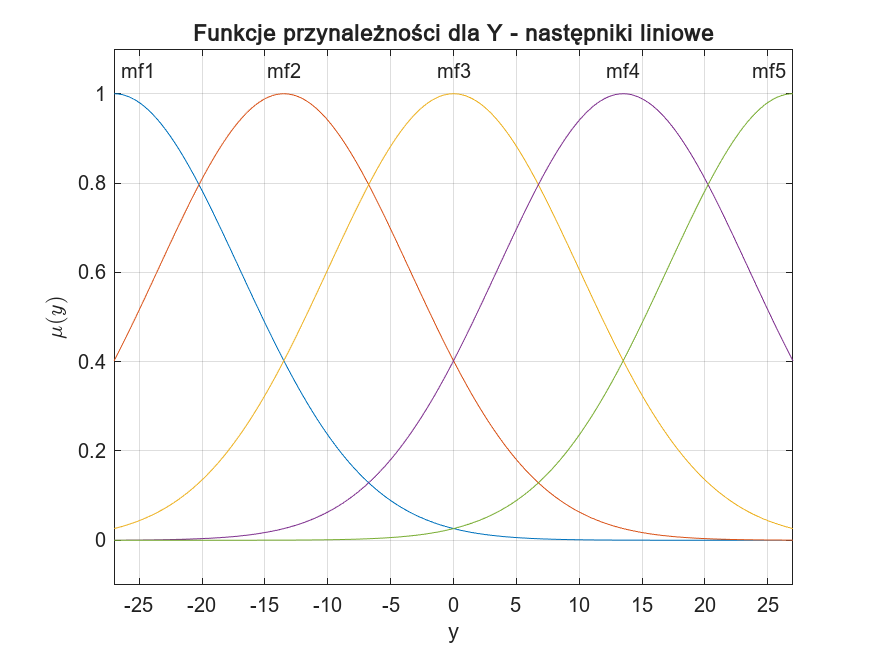
\includegraphics[width=\textwidth]{pictures/WienerfuzzySets_liniowe}
\caption{Zbiory rozmyte - model Wienera z następnikami liniowymi.}
\label{WienerfuzzySets_liniowe}
\end{figure}

\newpage

\section{Następniki nieliniowe}
Tak jak w poprzednim przypadku, w następnikach hiperbolicznych wykorzystano funkcję $\sinh$. 

\begin{equation}
\begin{array}{c}
\text{Jeśli } y \text{ jest } Y^1 \text{ to } y^1_{fuzzy}=a^1\sinh \left({\frac{y}{b^1}}\right) \\
\text{Jeśli } y \text{ jest } Y^2 \text{ to } y^2_{fuzzy}=a^2\sinh \left({\frac{y}{b^1}}\right) \\
\text{Jeśli } y \text{ jest } Y^3 \text{ to } y^3_{fuzzy}=a^3\sinh \left({\frac{y}{b^3}}\right) \\
\end{array}
\end{equation}

Po raz kolejny okazało się, że to właśnie odpowiednia normalizacja sygnału wyjściowego zapewnia satysfakcjonującą dokładność modelowania. Zbiory rozmyte dla modelu Wienera z następnikami nieliniowymi zaprezentowałem poniżej.

\begin{figure}[h!]
\centering
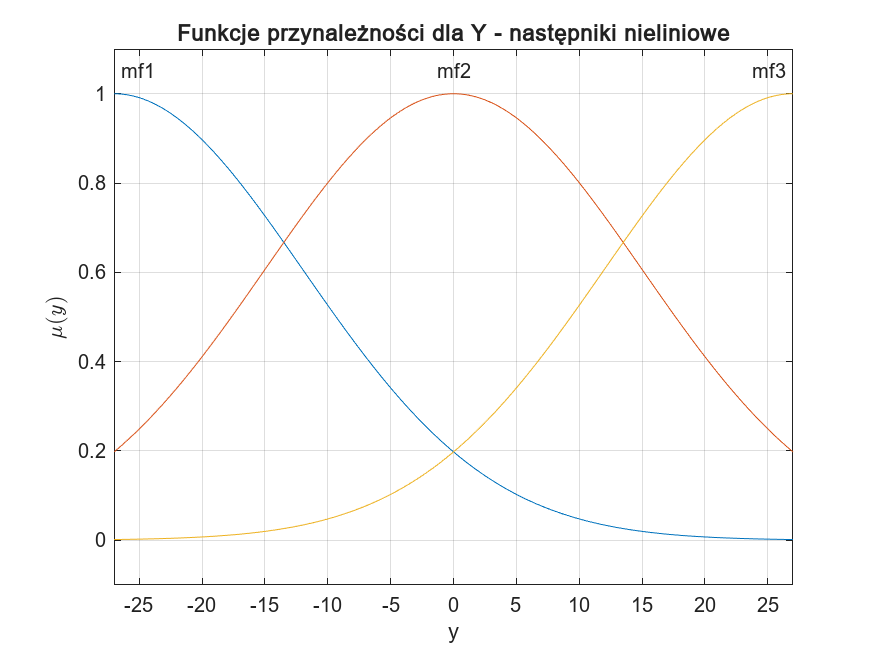
\includegraphics[width=\textwidth]{pictures/WienerfuzzySets_nieliniowe}
\caption{Zbiory rozmyte - model Wienera z następnikami nieliniowymi.}
\end{figure}